% 第5章第3节：线性映射（定义；表示：矩阵表示、基于矩阵的映射运算、矩阵基本子空间；核与像、秩零度、商空间、行空间与列空间、可逆性；换基：相抵与相似）。

\section{线性映射}
\label{sec:ls-linear-maps}
\label{sec:linear-algebra-matrices-linear-maps}

前两节研究的是单个空间中的对象怎样记录；本节转向对象之间的作用。一个作用要满足什么条件，才能用前两节的语言处理？选定基以后，它怎样记录成一张数表，两个作用叠加或接连进行时数表怎样变化？作用保留了哪些输入信息、丢失了哪些，什么时候可以由输出唯一反求输入？换一组基，记录同一个作用的数表怎样改变，哪些量不随之改变？本节的四个小节依次回答这四个问题。

\subsection{线性映射的定义}
\label{sec:ls-linear-map-definition}
\label{sec:linear-algebra-maps}

设计矩阵把一组系数变成一列拟合值，求导把一个多项式变成另一个多项式，读取第一个坐标把向量变成一个数。这些作用有一个共同点：输入先加权相加再作用，与先分别作用再作同样的加权相加，结果相同。正是这一点让前两节的语言可以用于作用本身：输入写成基向量的组合，作用就可以逐个基向量地计算。保持线性组合的作用称为\term{线性映射}（linear map）$T:V\to W$：
\begin{equation}
 T(a\bm x+b\bm y)=aT\bm x+bT\bm y,
 \qquad \bm x,\bm y\in V,\ a,b\in\mathbb R.
 \label{eq:ls-linear-map-def}
\end{equation}
取$a=b=0$得$T\bm0=\bm0$，线性映射总把原点留在原处。由式~\eqref{eq:prelim-matrix-linearity}，任何矩阵$\bm A\in\mathbb R^{m\times d}$给出的$\bm x\mapsto\bm A\bm x$都是从$\mathbb R^d$到$\mathbb R^m$的线性映射。下面再检查几个作用是否线性。
\begin{example}[线性与非线性的作用]
\label{ex:ls-linear-map-checks}
给定：三个作用
\[
 \begin{aligned}
 &T:\mathbb R^2\to\mathbb R^2, &&T(x_1,x_2)=(2x_1+x_2,\ 3x_2);\\
 &D:P_k\to P_k, &&Dp=p';\\
 &\tau:\mathbb R\to\mathbb R, &&\tau(x)=x+1.
 \end{aligned}
\]

验证：$T(x_1,x_2)$就是$\left[\begin{smallmatrix}2&1\\0&3\end{smallmatrix}\right]\bm x$，所以$T$保持线性组合。对多项式有$(ap+bq)'=ap'+bq'$，所以$D$保持线性组合；求导不升高次数，$D$确实把$P_k$送回$P_k$。$\tau(0)=1\neq0$，而线性映射必把$0$送到$0$。

结论：$T$与$D$是线性映射，$\tau$不是线性映射。
\end{example}

\phantomsection
\label{sec:ls-operator-powers}
输入与输出是同一个空间的线性映射$T:V\to V$称为\term{线性算子}（linear operator），也称线性变换。平面上的旋转、向一条直线的投影、$P_k$上的求导都是线性算子，示例~\ref{ex:ls-linear-map-checks}中的$T$也是。

算子是映射的特殊情形，但这一限制带来两点实质的不同。第一，输出仍在$V$中，可以再次作为输入，所以算子能与自身复合、反复作用：记$T^2=T\circ T$、$T^k=T\circ T^{k-1}$，并约定$T^0=\operatorname{id}_V$；一般映射$V\to W$在$V\neq W$时不能这样反复作用。下一小节将看到，在同一组基下，$T^k$的矩阵就是$T$的矩阵的$k$次幂。第二，记录算子时输入、输出可以用同一组基，这决定了算子换基时的特殊规律（第~\ref{sec:ls-similarity}节）。

\subsection{线性映射的表示（矩阵本质论）}
\label{sec:ls-map-representation}

线性映射的定义域通常有无穷多个元素，逐个记录输出是不可能的。本小节说明，有了基，有限个数就够了：在固定的两组基下，线性映射与矩阵一一对应，映射的叠加、复合与求逆分别对应矩阵的加法、乘法与求逆。第~\ref{chap:linear-operations}章的矩阵运算由此获得一般含义：矩阵就是线性映射在坐标下的记录。下面先建立这一对应，再把映射的运算翻译成矩阵的运算，最后对矩阵定义四个基本子空间，供下一小节计数信息的丢失与保留。

\subsubsection{矩阵表示}

给定输入基$\mathcal B=(\bm b_1,\ldots,\bm b_d)$，任一$\bm v=\sum_jx_j\bm b_j$的像由线性性写成
\[
 T\bm v=\sum_{j=1}^d x_j\,T\bm b_j,
\]
所以只要知道$d$个基向量的像，整个映射就确定了。再给定输出基$\mathcal C$，把每个像的坐标$[T\bm b_j]_{\mathcal C}$作为第$j$列，排成矩阵$\bm A=[T]_{\mathcal C\leftarrow\mathcal B}\in\mathbb R^{m\times d}$，称为$T$在这两组基下的矩阵。对上式两边取$\mathcal C$坐标，由坐标映射保持线性组合，并按矩阵与向量乘积的列读法，得到
\begin{equation}
 [T\bm v]_{\mathcal C}
 =\sum_{j=1}^d x_j\,[T\bm b_j]_{\mathcal C}
 =\sum_{j=1}^d x_j\bm A_{:,j}
 =[T]_{\mathcal C\leftarrow\mathcal B}\,[\bm v]_{\mathcal B}.
 \label{eq:linear-algebra-map-matrix-representation}
\end{equation}
也就是说，输出坐标等于矩阵乘以输入坐标：作用在对象上进行，记录在坐标上进行，二者由矩阵与向量的乘积连接。列数是输入维数，行数是输出维数；下标$\mathcal C\leftarrow\mathcal B$从右向左读，表示输入用$\mathcal B$记录、输出用$\mathcal C$记录。输入输出为同一空间的算子通常两端用同一组基，记为$[T]_{\mathcal B}=[T]_{\mathcal B\leftarrow\mathcal B}$，它是$\dim V$阶方阵。

下面按这一规则写出两个映射的矩阵。
\begin{example}[由基向量的像写出矩阵]
\label{ex:ls-plane-operator-matrix}
给定：示例~\ref{ex:ls-linear-map-checks}中的$T(x_1,x_2)=(2x_1+x_2,\ 3x_2)$，输入输出都取标准基。

计算：$T\bm e_1=(2,0)^{\top}$，$T\bm e_2=(1,3)^{\top}$。把它们依次作为两列，得
\[
 [T]=\begin{bmatrix}2&1\\0&3\end{bmatrix}.
\]

结论：$[T]$正是定义$T$时用的矩阵。
\end{example}
一般地，$\bm x\mapsto\bm A\bm x$在标准基下的矩阵就是$\bm A$本身，因为$\bm A\bm e_j=\bm A_{:,j}$。矩阵表示同样适用于不是数组的对象。
\begin{example}[求导的矩阵表示]
\label{ex:ls-derivative-matrix}
给定：求导$D:P_2\to P_2$，输入输出都取基$(1,t,t^2)$。

计算：$D1=0$，$Dt=1$，$Dt^2=2t$，三个像的坐标依次为$(0,0,0)^\top$、$(1,0,0)^\top$、$(0,2,0)^\top$，所以
\[
 [D]=\begin{bmatrix}0&1&0\\0&0&2\\0&0&0\end{bmatrix}.
\]
多项式$p=a_0+a_1t+a_2t^2$的坐标是$(a_0,a_1,a_2)^\top$，而$[D](a_0,a_1,a_2)^\top=(a_1,2a_2,0)^\top$，正是$p'=a_1+2a_2t$的坐标。

结论：对函数求导，在坐标下就是乘矩阵$[D]$。
\end{example}

\begin{theorem}[线性映射与矩阵的对应]
\label{thm:ls-map-matrix-correspondence}
设$\dim V=d$、$\dim W=m$，并固定$V$的基$\mathcal B$与$W$的基$\mathcal C$。则$T\mapsto[T]_{\mathcal C\leftarrow\mathcal B}$是从全部线性映射$V\to W$到全部$m\times d$实矩阵的双射。
\end{theorem}
\begin{proof}
单射：若两个线性映射的矩阵相同，它们在每个基向量上的像相同，由$T\bm v=\sum_jx_jT\bm b_j$，它们在每个$\bm v$上都相同。满射：任给$\bm A\in\mathbb R^{m\times d}$，对$\bm v\in V$令$T\bm v$为$\mathcal C$坐标等于$\bm A[\bm v]_{\mathcal B}$的那个向量。坐标唯一，所以这一规则有确定的意义；坐标映射与乘矩阵都保持线性组合，所以$T$线性；$T\bm b_j$的坐标是$\bm A\bm e_j=\bm A_{:,j}$，所以$[T]_{\mathcal C\leftarrow\mathcal B}=\bm A$。
\end{proof}
所以基固定以后，线性映射与矩阵一一对应；每个从$\mathbb R^d$到$\mathbb R^m$的线性映射在标准基下都等于乘某个矩阵。不过这一对应依赖基的选取：改变两端任一组基，通常会改变数表，而数表记录的仍是同一个映射。数表具体怎样随基改变，在第~\ref{sec:ls-coordinates-change-of-basis}节推导。

设计矩阵$\bm X_\varepsilon$正是这样一张记录：它表示$T_\varepsilon:\mathbb R^2\to\mathbb R^3$，$\bm w\mapsto\bm X_\varepsilon\bm w=w_1\bm c_1+w_2\bm c_2$，两列分别是两个输入基向量的像。输入是两个系数，输出是三个样本的拟合值，二者不能当成同一个空间中的向量。矩阵只是映射在两端坐标下的记录，不是映射本身的全部含义。图~\ref{fig:ch06-object-coordinate-map}中两条路径给出同一结果：先作用于对象再取坐标，与先取输入坐标再乘矩阵，得到相同的输出坐标。
\begin{figure}[htbp]
  \centering
  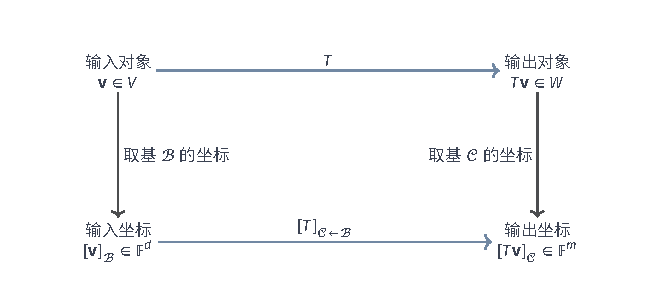
\includegraphics[width=112.0mm]{figures/00-shared/mathematical-preliminaries-upper/02-linear-spaces/tikz/ch06-object-coordinate-map/figure.pdf}
  \caption{先作用于对象再取坐标，与先取输入坐标再按矩阵的列作线性组合（即乘矩阵），得到相同输出坐标。横向箭头改变对象或数值，竖向箭头只改变记录方式。}
  \label{fig:ch06-object-coordinate-map}
\end{figure}

\subsubsection{基于矩阵的映射运算}
\phantomsection
\label{sec:ls-map-addition-composition}

两个映射可以把输出相加，也可以接连作用；一个映射可能可以撤销，也可能带上常数偏置。第~\ref{chap:linear-operations}章的矩阵加法、乘法与求逆，正是前三种运算在固定基下的记录；带偏置的仿射映射则可以借增广坐标写成一张更大的矩阵。

\paragraph{叠加}
\phantomsection
\label{sec:linear-algebra-map-addition}
设$T,S:V\to W$是同一对空间之间的两个线性映射，定义
\[
 (aT+bS)(\bm x)=aT\bm x+bS\bm x,\qquad \bm x\in V,
\]
其中$a,b\in\mathbb R$。叠加保持线性：把输入的线性组合代入，两个分支分别展开再汇总即可。在$V$与$W$的固定基下，若$T,S$的矩阵为$\bm A,\bm B$，则$aT+bS$把第$j$个基向量送到$aT\bm b_j+bS\bm b_j$，其坐标是$a\bm A_{:,j}+b\bm B_{:,j}$，所以$aT+bS$的矩阵就是$a\bm A+b\bm B$。

相加的前提是两个映射的定义域与陪域都一致。这并不要求$V=W$：两个从$\mathbb R^2$到$\mathbb R^3$的映射照样可以相加，只是不能与一个从$\mathbb R^3$到$\mathbb R^2$的映射相加；这对应于只有同形矩阵才能相加。系数$a,b$必须与输入无关；若叠加系数随$\bm x$改变，叠加后的映射一般不再线性，需要单独检验。

\paragraph{复合}
设$T:U\to V$、$S:V\to W$是线性映射。复合$S\circ T$先$T$后$S$，仍保持线性组合：$S(T(a\bm x+b\bm y))=S(aT\bm x+bT\bm y)=aS(T\bm x)+bS(T\bm y)$。取$U,V,W$的基$\mathcal B,\mathcal C,\mathcal D$，对每个$\bm x\in U$，两次使用式~\eqref{eq:linear-algebra-map-matrix-representation}，再用矩阵乘法的结合律，得
\[
 [S(T\bm x)]_{\mathcal D}
 =[S]_{\mathcal D\leftarrow\mathcal C}[T\bm x]_{\mathcal C}
 =[S]_{\mathcal D\leftarrow\mathcal C}\bigl([T]_{\mathcal C\leftarrow\mathcal B}[\bm x]_{\mathcal B}\bigr)
 =\bigl([S]_{\mathcal D\leftarrow\mathcal C}[T]_{\mathcal C\leftarrow\mathcal B}\bigr)[\bm x]_{\mathcal B}.
\]
取$\bm x=\bm b_j$，其坐标是$\bm e_j$，两边读出的是$[S\circ T]_{\mathcal D\leftarrow\mathcal B}$与乘积的第$j$列，所以
\begin{equation}
 [S\circ T]_{\mathcal D\leftarrow\mathcal B}
 =[S]_{\mathcal D\leftarrow\mathcal C}\,[T]_{\mathcal C\leftarrow\mathcal B}.
 \label{eq:ls-composition-matrix}
\end{equation}

复合的矩阵是矩阵的乘积，中间空间$V$的基$\mathcal C$在乘积中被消去；第~\ref{sec:prelim-linear-actions-composition}节的推导是这里取标准基的特例。恒等映射$\operatorname{id}_V$在同一组基下的矩阵是单位矩阵。于是映射复合的结合律与矩阵乘法的结合律互相对应，矩阵乘法不可交换，也就是先后作用的次序不能交换。

对算子$T:V\to V$两端都用基$\mathcal B$，反复使用式~\eqref{eq:ls-composition-matrix}，得$[T^k]_{\mathcal B}=([T]_{\mathcal B})^k$：算子的反复作用记录为第~\ref{sec:ls-matrix-power-rules}节的矩阵幂。例如对示例~\ref{ex:ls-derivative-matrix}中的$[D]$直接相乘可得$[D]^3=\bm0$，这对应于任何次数不超过$2$的多项式求导三次都变为零。

\paragraph{逆映射}
第~\ref{sec:prelim-inverse-matrices}节把满足$\bm A\bm B=\bm B\bm A=\bm I$的方阵$\bm A$称为可逆矩阵，那里只把它看成一次可以撤销的数表运算。有了矩阵表示，就可以问它记录的是哪一类映射。若线性映射$T:V\to W$是双射（第~\ref{chap:sets-functions-and-proofs}章~\ref{sec:prelim-function-types}节），每个输出恰有一个原输入，逆映射$T^{-1}:W\to V$存在。逆映射自动是线性的：对$\bm w,\bm w'\in W$，由$T$的线性性
\[
 T\bigl(aT^{-1}\bm w+bT^{-1}\bm w'\bigr)=a\bm w+b\bm w',
\]
所以$aT^{-1}\bm w+bT^{-1}\bm w'$就是$a\bm w+b\bm w'$唯一的原输入，即$T^{-1}(a\bm w+b\bm w')=aT^{-1}\bm w+bT^{-1}\bm w'$。这样的$T$称为可逆线性映射。

可逆映射与可逆矩阵是同一件事的两种记录。设$T:V\to W$可逆，在基$\mathcal B,\mathcal C$下$\bm A=[T]_{\mathcal C\leftarrow\mathcal B}$，$\bm B=[T^{-1}]_{\mathcal B\leftarrow\mathcal C}$。由式~\eqref{eq:ls-composition-matrix}，$T^{-1}\circ T=\operatorname{id}_V$与$T\circ T^{-1}=\operatorname{id}_W$分别给出$\bm B\bm A=\bm I$与$\bm A\bm B=\bm I$，所以$\bm A$是可逆方阵（下一小节将说明此时必有$\dim V=\dim W$），且$[T^{-1}]_{\mathcal B\leftarrow\mathcal C}=\bm A^{-1}$。反过来，若$\bm A$可逆，$\bm y\mapsto\bm A^{-1}\bm y$就是$\bm x\mapsto\bm A\bm x$的逆映射。

两个可逆映射接连作用时，$(S\circ T)^{-1}=T^{-1}\circ S^{-1}$，在矩阵上就是式~\eqref{eq:ls-inverse-product}。至于一个映射什么时候可逆，要先弄清它丢失了什么、能到达什么，这是下一小节的内容。

\paragraph{仿射映射}
\phantomsection
\label{sec:ls-affine-maps}
线性模型的预测常带截距，平面上的平移也常与旋转一起出现，它们都不把原点留在原处。这样的作用怎样纳入线性映射的框架？带常数偏置的规则$\bm x\mapsto\bm A\bm x+\bm b$在$\bm b\neq\bm0$时称为\term{仿射映射}（affine map）。它不是线性映射：它把$\bm0$送到$\bm b$，而线性映射必将$\bm0$送到$\bm0$。两个仿射映射$\bm x\mapsto\bm A_1\bm x+\bm b_1$、$\bm y\mapsto\bm A_2\bm y+\bm b_2$复合得$\bm x\mapsto\bm A_2\bm A_1\bm x+(\bm A_2\bm b_1+\bm b_2)$，前一个映射的平移项也被后一个映射作用。

给坐标补一个恒为$1$的末位，仿射映射可以写成高一维空间上的线性作用：
\begin{equation}
 \begin{bmatrix}\bm A&\bm b\\ \bm0^\top&1\end{bmatrix}
 \begin{bmatrix}\bm x\\1\end{bmatrix}
 =
 \begin{bmatrix}\bm A\bm x+\bm b\\1\end{bmatrix}.
 \label{eq:ls-affine-homogeneous}
\end{equation}
按分块乘法，两个这样的增广矩阵相乘得
\[
 \begin{bmatrix}\bm A_2&\bm b_2\\ \bm0^\top&1\end{bmatrix}
 \begin{bmatrix}\bm A_1&\bm b_1\\ \bm0^\top&1\end{bmatrix}
 =\begin{bmatrix}\bm A_2\bm A_1&\bm A_2\bm b_1+\bm b_2\\ \bm0^\top&1\end{bmatrix},
\]
正是复合仿射映射的增广矩阵。

大矩阵对整个增广空间是线性的，但原输入被限制在末坐标为$1$的集合上，不能据此声称原映射线性。第~\ref{chap:linear-equations-and-optimization}章用这种形式描述仿射解集的几何。

\subsubsection{矩阵基本子空间}
\phantomsection
\label{sec:ls-four-fundamental-subspaces}

一张矩阵$\bm A\in\mathbb R^{m\times d}$既给出从$\mathbb R^d$到$\mathbb R^m$的映射$\bm x\mapsto\bm A\bm x$，它的转置$\bm A^\top\in\mathbb R^{d\times m}$又给出反方向的映射$\bm y\mapsto\bm A^\top\bm y$。对每个方向问两个问题：哪些输出可以到达，哪些输入被送到零。四个答案都是子空间，它们刻画了矩阵怎样保留和丢失信息。

按矩阵与向量乘积的列读法，$\bm A\bm x=\sum_jx_j\bm A_{:,j}$；$\bm x$取遍$\mathbb R^d$时，输出取遍$\bm A$各列的全部线性组合，即各列的张成空间，称为$\bm A$的\term{列空间}（column space），记为$\operatorname{range}(\bm A)$。所以方程$\bm A\bm x=\bm b$有解当且仅当$\bm b\in\operatorname{range}(\bm A)$。

齐次方程组$\bm A\bm x=\bm0$的解集合是$\mathbb R^d$的子空间（示例~\ref{ex:ls-subspace-checks}），称为$\bm A$的\term{零空间}（null space），记为$\operatorname{null}(\bm A)$。对$\bm A^\top$问同样的两个问题，又得到两个子空间。$\bm A^\top$的列就是$\bm A$的行（竖排），所以$\operatorname{range}(\bm A^\top)$由$\bm A$各行的线性组合组成，称为$\bm A$的\term{行空间}（row space）。$\bm A^\top\bm y=\bm0$转置后就是$\bm y^\top\bm A=\bm0^\top$：$\bm y^\top$从左边乘上$\bm A$得到零，所以$\operatorname{null}(\bm A^\top)$称为$\bm A$的\term{左零空间}（left null space）。这四个子空间合称$\bm A$的\term{四个基本子空间}（four fundamental subspaces）：
\begin{equation}
 \begin{aligned}
  \operatorname{range}(\bm A)&=\{\bm A\bm x:\bm x\in\mathbb R^d\}\subseteq\mathbb R^m,\\
  \operatorname{null}(\bm A)&=\{\bm x\in\mathbb R^d:\bm A\bm x=\bm0\}\subseteq\mathbb R^d,\\
  \operatorname{range}(\bm A^\top)&=\{\bm A^\top\bm y:\bm y\in\mathbb R^m\}\subseteq\mathbb R^d,\\
  \operatorname{null}(\bm A^\top)&=\{\bm y\in\mathbb R^m:\bm A^\top\bm y=\bm0\}\subseteq\mathbb R^m.
 \end{aligned}
 \label{eq:ls-four-fundamental-subspaces}
\end{equation}

零空间与行空间在输入空间$\mathbb R^d$中，列空间与左零空间在输出空间$\mathbb R^m$中。零空间收集被完全消去的输入方向。行空间收集读取输出分量所用的方向：输出的第$i$个分量$(\bm A\bm x)_i=\bm A_{i,:}\bm x$是第$i$行与$\bm x$逐项相乘再相加。左零空间收集对可达输出的“盲读”：对$\bm y\in\operatorname{null}(\bm A^\top)$与任意输入$\bm x$，$\bm y^\top(\bm A\bm x)=(\bm y^\top\bm A)\bm x=0$，即用$\bm y$对可达输出加权求和，结果总是零。

下面对一个具体矩阵求出四个基本子空间。
\begin{example}[一个$2\times3$矩阵的四个基本子空间]
\label{ex:ls-rank-one-four-subspaces}
给定：
\[
 \bm A=\begin{bmatrix}1&2&3\\2&4&6\end{bmatrix}\in\mathbb R^{2\times3}.
\]

计算：列空间：三列$(1,2)^\top$、$(2,4)^\top$、$(3,6)^\top$都是$(1,2)^\top$的倍数，所以$\operatorname{range}(\bm A)=\operatorname{span}\{(1,2)^\top\}$，是$\mathbb R^2$中的直线。零空间：第二行是第一行的$2$倍，$\bm A\bm x=\bm0$只剩一个方程$x_1+2x_2+3x_3=0$，由示例~\ref{ex:ls-solution-plane-basis}，$\operatorname{null}(\bm A)=\operatorname{span}\{(-2,1,0)^\top,(-3,0,1)^\top\}$，是$\mathbb R^3$中的平面。行空间：两行都是$(1,2,3)$的倍数，所以$\operatorname{range}(\bm A^\top)=\operatorname{span}\{(1,2,3)^\top\}$，是$\mathbb R^3$中的直线。左零空间：$\bm y^\top\bm A=(y_1+2y_2)(1,2,3)$为零当且仅当$y_1=-2y_2$，所以$\operatorname{null}(\bm A^\top)=\operatorname{span}\{(2,-1)^\top\}$，是$\mathbb R^2$中的直线。

结论：列空间、零空间、行空间、左零空间的维数依次为$1,2,1,1$。列空间与行空间维数相同；输入空间中零空间与行空间的维数之和为$2+1=3$，输出空间中列空间与左零空间的维数之和为$1+1=2$。此外，行空间的方向$(1,2,3)^\top$与零空间的两个基向量逐项相乘再相加都得零（$-2+2+0=0$，$-3+0+3=0$），列空间的方向$(1,2)^\top$与左零空间的方向$(2,-1)^\top$也是如此（$2-2=0$）。
\end{example}
第~\ref{sec:ls-kernel-image}节说明，示例中的两条维数规律对任何矩阵都成立；垂直关系则要等第~\ref{sec:ls-orthogonality}节有了内积以后才能说清。

\subsection{核与像}
\label{sec:ls-kernel-image}

一个映射丢失了哪些输入信息，又能产生哪些输出？这两个问题决定了能否由输出反求输入。本小节先把它们写成两个子空间，再用秩零度定理说明二者的维数此消彼长，并用商空间重新解读这一关系；然后求出矩阵四个基本子空间的维数；最后给出单射、满射与可逆的判据。

\paragraph{核与像}
被映射送到零的输入集合称为$T$的核（kernel），记为$\ker T=\{\bm x\in V:T\bm x=\bm0\}$；所有可到达的输出集合称为\term{像空间}（简称像，image），记为$\operatorname{im}T=\{T\bm x:\bm x\in V\}$。二者都是子空间：若$T\bm x=T\bm y=\bm0$，则$T(a\bm x+b\bm y)=\bm0$；若$\bm u=T\bm x$、$\bm v=T\bm y$，则$a\bm u+b\bm v=T(a\bm x+b\bm y)$。

核记录被映射完全消去的输入方向，像记录可达的输出范围；二者分别位于输入端与输出端，不能当作同一空间中的两个集合直接比较。对矩阵$\bm A\in\mathbb R^{m\times d}$，映射$\bm x\mapsto\bm A\bm x$的核就是零空间$\operatorname{null}(\bm A)$，像就是列空间$\operatorname{range}(\bm A)$（第~\ref{sec:ls-four-fundamental-subspaces}节）。说“矩阵$\bm A$的核”“矩阵$\bm A$的秩”时，指的都是映射$\bm x\mapsto\bm A\bm x$的相应量。

核为什么代表“丢失的信息”？因为$T\bm x=T\bm y$当且仅当$T(\bm x-\bm y)=\bm0$，即$\bm x-\bm y\in\ker T$：两个输入相差一个核方向时，输出完全相同。下面的例子用三个响应读取四个分量，展示这一点。
\begin{example}[相差核方向的输入给出相同输出]
\label{ex:ls-kernel-indistinguishable}
给定：$T:\mathbb R^4\to\mathbb R^3$，
\[
 T(x_1,x_2,x_3,x_4)=(x_1+x_4,\ x_2+x_4,\ x_3+x_4).
\]

计算：$T\bm x=\bm0$当且仅当$x_1=x_2=x_3=-x_4$，所以$\ker T=\operatorname{span}\{(1,1,1,-1)^{\top}\}$。取$x_4=0$时，$T\bm x=(x_1,x_2,x_3)$可以是任意向量，所以$\operatorname{im}T=\mathbb R^3$。两个输入$(1,1,1,1)^\top$与$(0,0,0,2)^\top$之差为$(1,1,1,-1)^\top\in\ker T$，相应地
\[
 T(1,1,1,1)=T(0,0,0,2)=(2,2,2).
\]

结论：仅凭三个响应无法区分这两个输入，也无法区分任何两个相差$(1,1,1,-1)^\top$倍数的输入。
\end{example}
这就是线性不可辨识性：两个输入相差核方向时输出相同，只凭输出无法确定输入。若另有约束限制了可取的输入，能否辨识还要结合这些约束判断。

\paragraph{秩零度定理}
\phantomsection
\label{sec:ls-rank-nullity}
核与像各有多大？二者的维数之间有一条精确的守恒关系。像的维数称为\term{秩}（rank）$\operatorname{rank}T=\dim\operatorname{im}T$，核的维数称为\term{零度}（nullity）$\dim\ker T$。
\begin{theorem}[秩零度定理]
\label{thm:ls-rank-nullity}
\label{thm:linear-algebra-rank-nullity}
有限维线性映射$T:V\to W$满足
\begin{equation}
 \dim V=\dim\ker T+\dim\operatorname{im}T,
 \qquad\text{即}\qquad
 \dim V=\dim\ker T+\operatorname{rank}T.
 \label{eq:ls-rank-nullity}
\end{equation}
\end{theorem}
\begin{proof}
取核的一组基$\bm v_1,\ldots,\bm v_r$并扩充成$V$的基$\bm v_1,\ldots,\bm v_d$。前$r$个基向量的像为零，所以其余像$T\bm v_{r+1},\ldots,T\bm v_d$张成像。若$\sum_{j>r}a_jT\bm v_j=\bm0$，则$\sum_{j>r}a_j\bm v_j$属于核，能由前$r$个基向量表示；整个基的线性无关性迫使全部$a_j=0$，所以这些像也是无关组。像的维数为$d-r$，结论成立。
\end{proof}
对矩阵$\bm A\in\mathbb R^{m\times d}$，记$\operatorname{rank}\bm A$为其映射的秩，即列空间的维数，有$d=\dim\operatorname{null}(\bm A)+\operatorname{rank}\bm A$。秩计数独立的输出方向，零度计数被消去的独立输入方向，二者此消彼长。在示例~\ref{ex:ls-kernel-indistinguishable}中，$\dim\ker T=1$、$\operatorname{rank}T=3$，二者之和为输入维数$4$。图~\ref{fig:ls-kernel-image-rank-nullity}再给出两个几何化算例：被映到零的方向与实际用到的输出方向，维数相加恰为定义域维数。
\begin{figure*}[htbp]
  \centering
  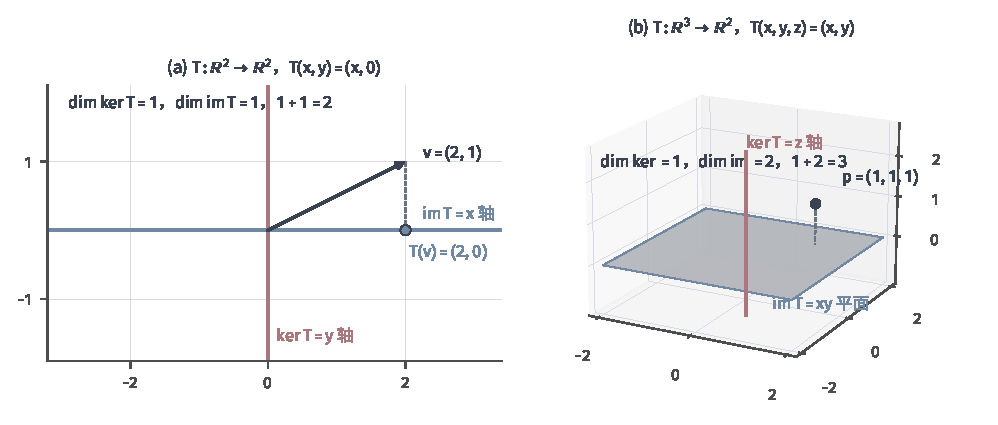
\includegraphics[width=169mm]{figures/00-shared/mathematical-preliminaries-upper/02-linear-spaces/matplotlib/ls-kernel-image-rank-nullity/ls-kernel-image-rank-nullity.pdf}
  \caption{核与像的维数此消彼长。左：$T(x,y)=(x,0)$把平面映到$x$轴，核是$y$轴（红直线）、像是$x$轴（蓝直线），$\dim\ker T=1$、$\dim\operatorname{im}T=1$，$1+1=2$；样本$\bm v=(2,1)$被映到$(2,0)$。右：$T(x,y,z)=(x,y)$把三维空间映到$xy$平面，核是$z$轴（红直线）、像是整个$xy$平面（浅蓝），$\dim\ker T=1$、$\dim\operatorname{im}T=2$，$1+2=3$。两图为解析教学例。}
  \label{fig:ls-kernel-image-rank-nullity}
\end{figure*}

对$\bm A\in\mathbb R^{m\times d}$，$\operatorname{rank}\bm A\leq\min(m,d)$：列空间在$\mathbb R^m$中，维数不超过$m$；它由$d$列张成，从中抽取出的基不超过$d$个向量。$\operatorname{rank}\bm A=d$称为满列秩，这时输入方向全部被保留，等价于各列线性无关；$\operatorname{rank}\bm A=m$称为满行秩，这时输出全部可达；二者统称\term{满秩}（full rank）。

形状不同时，二者不能同时成立。$m<d$时，即使满行秩，核的维数也是$d-m>0$；$m>d$时，即使满列秩，像的维数也只有$d<m$，总有输出无法到达。例如贯穿例$\bm X_\varepsilon$在$\varepsilon\neq0$时两列线性无关（示例~\ref{ex:ls-nearly-collinear-independence}），秩为$2$，满列秩；它的像是$\mathbb R^3$中的一个平面，不是满行秩。

\paragraph{商空间}
前面看到，输出相同的输入恰好彼此相差一个核方向。按输出把输入分组，每组都形如$\bm x+\ker T$，正是第~\ref{sec:ls-quotient-spaces}节取$U=\ker T$得到的等价类，全部分组组成商空间$V/\ker T$。

规则$\bm x+\ker T\mapsto T\bm x$不依赖代表元，因为代表元相差核方向时输出相同。它保持线性组合，满射到$\operatorname{im}T$；它也是单射，因为两个类的像相同即$T\bm x=T\bm y$时，$\bm x-\bm y\in\ker T$，两个类相同。所以它是从$V/\ker T$到$\operatorname{im}T$的线性双射：压去全部丢失方向以后，每个等价类恰对应一个可达输出。线性双射把一组基送到一组基，两边维数相同；由式~\eqref{eq:ls-quotient-dimension}得$\dim V-\dim\ker T=\operatorname{rank}T$，这是秩零度定理的另一种读法。在示例~\ref{ex:ls-kernel-indistinguishable}中，商空间$\mathbb R^4/\ker T$是三维的，像$\mathbb R^3$也是三维的。

\paragraph{矩阵的行空间与列空间}
示例~\ref{ex:ls-rank-one-four-subspaces}中，行空间与列空间维数相同，零空间与行空间的维数之和为输入维数，列空间与左零空间的维数之和为输出维数。现在对一般的$\bm A\in\mathbb R^{m\times d}$证明这些规律。对$\bm A$用秩零度定理，零空间与列空间的维数之和为$d$；对$\bm A^\top$用它，左零空间与行空间的维数之和为$m$。剩下的问题是两个“列空间”之间的关系：行空间与列空间是否总一样大？
\begin{theorem}[行秩等于列秩]
\label{thm:ls-row-rank-column-rank}
对任意$\bm A\in\mathbb R^{m\times d}$，$\dim\operatorname{range}(\bm A^\top)=\dim\operatorname{range}(\bm A)$，即$\operatorname{rank}\bm A^\top=\operatorname{rank}\bm A$。
\end{theorem}
\begin{proof}
设$r=\operatorname{rank}\bm A$，取列空间的一组基$\bm c_1,\ldots,\bm c_r$，排成$\bm C\in\mathbb R^{m\times r}$。$\bm A$的每一列都在列空间中，所以第$j$列可写成$\bm A_{:,j}=\bm C\bm r_j$，$\bm r_j\in\mathbb R^r$；把这些系数列排成$\bm R\in\mathbb R^{r\times d}$，按乘积的列读法得$\bm A=\bm C\bm R$。再按行读这个乘积：$\bm A$的第$i$行是$\bm A_{i,:}=\sum_{k=1}^r\bm C_{i,k}\bm R_{k,:}$，即$\bm R$的$r$行的线性组合。所以$\bm A$的全部行都落在$\bm R$的$r$行张成的空间里，行空间的维数不超过$r$，即$\operatorname{rank}\bm A^\top\leq\operatorname{rank}\bm A$。对$\bm A^\top$用同样的论证，得$\operatorname{rank}\bm A\leq\operatorname{rank}\bm A^\top$，两者相等。
\end{proof}
于是行秩（行空间的维数）与列秩（列空间的维数）可以统称为秩。对$\bm A$与$\bm A^\top$分别用秩零度定理，四个基本子空间的维数全部由$m,d$与$r=\operatorname{rank}\bm A$决定：
\begin{equation}
 \begin{gathered}
 \dim\operatorname{range}(\bm A)=\dim\operatorname{range}(\bm A^\top)=r,\\
 \dim\operatorname{null}(\bm A)=d-r,\qquad
 \dim\operatorname{null}(\bm A^\top)=m-r.
 \end{gathered}
 \label{eq:ls-four-subspace-dimensions}
\end{equation}
输入空间中的零空间与行空间维数相加为$d$，输出空间中的列空间与左零空间维数相加为$m$。

对示例~\ref{ex:ls-rank-one-four-subspaces}中的$\bm A$，$r=1$，式~\eqref{eq:ls-four-subspace-dimensions}给出的维数与直接计算一致；证明中的分解$\bm A=\bm C\bm R$在那里就是$\bm A=(1,2)^\top(1,2,3)$。该示例还显示，两对子空间不仅维数互补，而且互相垂直。这一规律要在第~\ref{sec:ls-orthogonality}节有了内积以后才能说清；第~\ref{sec:ls-dual-map}节还将用对偶映射给出行秩等于列秩的另一个证明。

\paragraph{单射、满射与可逆性}
\phantomsection
\label{sec:ls-injective-surjective-invertible}
给定输出，能否唯一还原输入？这个问题分成两半：不同的输入是否给出不同的输出，以及每个输出是否都能被到达。对线性映射，这两半都可以用子空间判断。单射等价于核为零：$T\bm x=T\bm y$当且仅当$\bm x-\bm y\in\ker T$，核为零时输出相同必输入相同；反过来，核中若有非零向量，它与$\bm0$的输出相同，映射就不是单射。满射等价于像等于整个输出空间。有限维时可以用秩零度定理把二者换成维数：单射当且仅当$\operatorname{rank}T=\dim V$，满射当且仅当$\operatorname{rank}T=\dim W$。

输入输出维数相等时，秩零度定理使三种性质合而为一：$\dim V=\dim W$时，$\ker T=\{\bm0\}$等价于$\operatorname{rank}T=\dim V=\dim W$，于是单射、满射、双射互相等价，只需检查其中一条。维数不同时则须分别判断：$\dim V<\dim W$时像的维数至多为$\dim V$，不可能满射；$\dim V>\dim W$时核的维数至少为$\dim V-\dim W>0$，不可能单射。所以只有输入输出维数相等的映射才可能双侧可逆，矩形矩阵即使满秩，也只能是单射或满射之一。

把这些判据与上一小节可逆映射和逆矩阵的对应合起来，对$n$阶方阵$\bm A$，下列条件互相等价：
\[
 \bm A\text{可逆}
 \iff\operatorname{null}(\bm A)=\{\bm0\}
 \iff\operatorname{rank}\bm A=n
 \iff\bm A\text{的}n\text{列线性无关}.
\]
其中第三、四个条件等价，是因为列空间由$n$列张成，维数为$n$恰好说明这$n$列构成它的一组基。由行秩等于列秩，还可以在链中加入“$\bm A$的$n$行线性无关”。第~\ref{sec:ls-determinant-invertibility}节讨论线性方程时，还将用行列式给出一个等价的数值判据$\det\bm A\neq0$。

这一等价还给出第~\ref{sec:ls-square-one-sided-inverse}节“方阵的单侧逆即逆”的另一个证明，不必借助行列式。若$n$阶方阵满足$\bm B\bm A=\bm I_n$，则$\bm A\bm x=\bm0$蕴含$\bm x=\bm B\bm A\bm x=\bm0$，核为零，$\bm A$可逆，于是$\bm B=\bm B\bm A\bm A^{-1}=\bm A^{-1}$；$\bm A\bm B=\bm I_n$时对$\bm B$作同样论证。

同理，若$n$阶方阵的乘积$\bm A\bm B$可逆，则两个因子都可逆。$\bm B\bm x=\bm0$蕴含$\bm A\bm B\bm x=\bm0$，从而$\bm x=\bm0$，$\bm B$的核为零，因而可逆；于是$\bm A=(\bm A\bm B)\bm B^{-1}$是可逆矩阵的乘积，也可逆。

最容易还原的情形是逐坐标缩放；一般的矩阵把坐标掺在一起，但判据相同：核为零且维数相等。
\begin{example}[用核判断可逆]
\label{ex:ls-kernel-invertibility}
给定：对角矩阵$\operatorname{diag}(d_1,\ldots,d_n)$与$\bm A=\left[\begin{smallmatrix}2&1\\0&3\end{smallmatrix}\right]$。

验证：对角矩阵逐坐标缩放，坐标之间互不影响。若每个$d_i\neq0$，逐坐标除以$d_i$即可撤销，逆矩阵为$\operatorname{diag}(1/d_1,\ldots,1/d_n)$。若某个$d_i=0$，相应坐标被压为零，$\bm e_i$落入核中，两个只在第$i$个坐标不同的输入给出相同输出。对$\bm A$，$\bm A\bm x=\bm0$即$2x_1+x_2=0$与$3x_2=0$；第二式给出$x_2=0$，代入第一式得$x_1=0$，所以核为零。

结论：对角矩阵可逆当且仅当全部$d_i\neq0$；$\bm A$是方阵且核为零，所以可逆，它的逆矩阵已在第~\ref{sec:prelim-inverse-matrices}节求出。
\end{example}

\paragraph{单侧逆}
维数不同时，仍可以只撤销一半。单射$T:V\to W$可以找到线性映射$L:W\to V$使$L\circ T=\operatorname{id}_V$：在像上按$T$的逆读回输入，在像的一个补空间上任意规定（例如送到零）。满射$T$可以找到$R:W\to V$使$T\circ R=\operatorname{id}_W$：为输出基中的每个向量任选一个原输入，再线性延拓。补空间与原输入的选法不唯一，所以这些单侧逆一般也不唯一。

写成矩阵，对$\bm A\in\mathbb R^{m\times d}$：$\bm A$有左逆当且仅当它满列秩，有右逆当且仅当它满行秩。充分性来自上面的构造，因为满列秩就是单射，满行秩就是满射。必要性同样直接：若$\bm L\bm A=\bm I_d$，则$\bm A\bm x=\bm0$蕴含$\bm x=\bm L\bm A\bm x=\bm0$，核为零；若$\bm A\bm R=\bm I_m$，则每个$\bm y=\bm A(\bm R\bm y)$都可到达。第~\ref{sec:prelim-inverse-matrices}节的例子$\bm A=(1,0)^\top$满列秩，有无穷多个左逆。多解时如何选择代表，由第~\ref{chap:linear-equations-and-optimization}章回答。

\subsection{线性映射的换基}
\label{sec:ls-coordinates-change-of-basis}

第~\ref{sec:ls-coordinates}节看到，同一个对象在不同基下有不同的坐标；同样，同一个线性映射换一组基，记录它的矩阵通常也随之改变。现在坐标变换、矩阵表示与逆矩阵都已齐备，这种变化可以精确写出。本小节回答两个问题：一般线性映射在输入、输出两端各自换基以后，矩阵怎样变化，两个同形矩阵什么时候记录同一个映射；线性算子两端一起换基时，又会怎样。

一般映射放在算子之前。映射的两端是两个空间，可以独立换基，得到的关系称为相抵；算子要求两端使用同一组基，换基时两端必须一起变，相应的关系称为相似，它是相抵加上“两端换基相同”这一约束的特例。约束减少了可用的自由度：相抵只需秩就能完全分类，相似却要更多不变量。

推导要用到一个观察：换基矩阵本身就是一个线性映射的矩阵。比较式~\eqref{eq:linear-algebra-coordinate-change}与式~\eqref{eq:linear-algebra-map-matrix-representation}可见，$\bm S_{\mathcal C\leftarrow\mathcal B}$正是恒等映射$\operatorname{id}_V$在输入基$\mathcal B$、输出基$\mathcal C$下的矩阵：对象不动，只是输入端与输出端用不同的基记录。连续换基的乘法公式，也就是复合公式~\eqref{eq:ls-composition-matrix}对$\operatorname{id}_V\circ\operatorname{id}_V=\operatorname{id}_V$的特例。

\subsubsection{一般线性映射的换基与相抵}
\label{sec:ls-equivalence-matrices}

设$T:V\to W$是线性映射，$\dim V=d$、$\dim W=m$。它在一对基下记录为矩阵$\bm A$，在另一对基下记录为$\bm B$，$\bm A$与$\bm B$有什么关系？反过来，两个同形矩阵什么时候记录的是同一个映射？

\paragraph{换基过程}
设$\mathcal B,\mathcal B'$是$V$的两组基，$\mathcal C,\mathcal C'$是$W$的两组基，记$\bm A=[T]_{\mathcal C\leftarrow\mathcal B}$、$\bm B=[T]_{\mathcal C'\leftarrow\mathcal B'}$，输入端换基矩阵$\bm P=\bm S_{\mathcal B\leftarrow\mathcal B'}$（$d$阶可逆），输出端换基矩阵$\bm Q=\bm S_{\mathcal C\leftarrow\mathcal C'}$（$m$阶可逆）。$\bm P$的第$j$列是新输入基向量在旧输入基下的坐标，$\bm Q$同理。已知新输入坐标$[\bm v]_{\mathcal B'}$，求新输出坐标$[T\bm v]_{\mathcal C'}$，可以绕道旧基分三步完成。

第一步，把新输入坐标换成旧输入坐标：$[\bm v]_{\mathcal B}=\bm P[\bm v]_{\mathcal B'}$。第二步，在旧基下作用：$[T\bm v]_{\mathcal C}=\bm A[\bm v]_{\mathcal B}=\bm A\bm P[\bm v]_{\mathcal B'}$。第三步，把旧输出坐标换成新输出坐标，这要用反向换基矩阵$\bm Q^{-1}=\bm S_{\mathcal C'\leftarrow\mathcal C}$：
\[
 [T\bm v]_{\mathcal C'}=\bm Q^{-1}[T\bm v]_{\mathcal C}=\bm Q^{-1}\bm A\bm P[\bm v]_{\mathcal B'}.
\]
另一方面，按定义$[T\bm v]_{\mathcal C'}=\bm B[\bm v]_{\mathcal B'}$。两式对每个$\bm v$成立；取$\bm v=\bm b'_j$，其新坐标为$\bm e_j$，两边读出的是两个矩阵的第$j$列，所以
\begin{equation}
 \bm B=\bm Q^{-1}\bm A\bm P.
 \label{eq:ls-equivalence-transform}
\end{equation}
从右向左读：$\bm P$把新输入坐标译成旧坐标，$\bm A$在旧基下作用，$\bm Q^{-1}$把结果译成新输出坐标。用复合的语言说，$T=\operatorname{id}_W\circ T\circ\operatorname{id}_V$，三个因子分别在相应的基下记录，由式~\eqref{eq:ls-composition-matrix}就是上式右端的三个矩阵。

\paragraph{相抵的定义}
\phantomsection
\label{sec:ls-equivalence-meaning}
上面的推导说明，同一映射的两个记录之间只相差两侧各乘一个可逆矩阵。反过来，两侧任意乘上可逆矩阵，得到的是否仍是同一映射的记录？先把这种关系单独命名。
\begin{definition}[矩阵相抵]
\label{def:ls-matrix-equivalence}
设$\bm A,\bm B\in\mathbb R^{m\times d}$。若存在可逆矩阵$\bm Q\in\mathbb R^{m\times m}$与$\bm P\in\mathbb R^{d\times d}$使$\bm B=\bm Q^{-1}\bm A\bm P$，就称$\bm A$与$\bm B$\term{相抵}（equivalent matrices）。
\end{definition}
定义中的$\bm Q,\bm P$可以是任意可逆矩阵，不必事先知道它们来自哪组基；写成$\bm Q^{-1}$只是为了与换基推导一致，$\bm Q$取遍全部可逆矩阵时$\bm Q^{-1}$也取遍全部可逆矩阵。

相抵恰好刻画“记录同一个映射”。一个方向已由换基推导给出。另一方向，设$\bm A=[T]_{\mathcal C\leftarrow\mathcal B}$，任给可逆的$\bm P,\bm Q$。由第~\ref{sec:ls-coordinates}节，以$\bm P$的各列为旧基坐标可以得到$V$的一组新基$\mathcal B'$，使$\bm S_{\mathcal B\leftarrow\mathcal B'}=\bm P$；输出端用$\bm Q$同样构造$\mathcal C'$。由换基推导，$T$在这两组新基下的矩阵恰为$\bm Q^{-1}\bm A\bm P$。所以两个同形矩阵相抵，当且仅当它们是同一个线性映射在两端不同选基下的记录。右乘$\bm P$对应输入基的更换，左乘$\bm Q^{-1}$对应输出基的更换；初等列变换与初等行变换分别是这两种换基的具体实现。

\paragraph{相抵不变量}
\phantomsection
\label{sec:ls-equivalence-properties}
既然相抵的矩阵记录同一个映射，映射本身的性质就不应随基改变。哪些量是这样的不变量？相抵首先是等价关系：自反取$\bm Q=\bm P=\bm I$；对称由$\bm A=\bm Q\bm B\bm P^{-1}=(\bm Q^{-1})^{-1}\bm B\bm P^{-1}$；传递由$\bm C=\bm Q_2^{-1}\bm B\bm P_2=(\bm Q_1\bm Q_2)^{-1}\bm A(\bm P_1\bm P_2)$。三条分别对应不换基、换回原基和连续换两次基。

零空间在输入端被搬运：$\bm B\bm x=\bm0$当且仅当$\bm A(\bm P\bm x)=\bm0$，所以$\operatorname{null}(\bm B)=\bm P^{-1}\operatorname{null}(\bm A)$。列空间在输出端被搬运：$\bm B\bm x=\bm Q^{-1}\bm A(\bm P\bm x)$，而$\bm P\bm x$取遍全部输入，所以$\operatorname{range}(\bm B)=\bm Q^{-1}\operatorname{range}(\bm A)$。可逆矩阵把线性无关组送到线性无关组，搬运不改变子空间的维数，因此
\begin{equation}
 \operatorname{rank}\bm B=\operatorname{rank}\bm A,
 \qquad
 \dim\operatorname{null}(\bm B)=\dim\operatorname{null}(\bm A)=d-\operatorname{rank}\bm A.
 \label{eq:ls-equivalence-invariants}
\end{equation}
相抵允许的记录变化很宽：输入与输出可以是不同空间，$\bm B$一般不是方阵，不能对自身反复作用，所以幂、迹这类只对算子有意义的量不在讨论之列。

\paragraph{秩标准形与相抵判据}
\phantomsection
\label{sec:ls-equivalence-conditions}
秩是相抵不变量；反过来，秩相同的两个同形矩阵是否一定相抵？答案是肯定的。办法是说明两端可以独立选基时，每个矩阵都能化成只由秩决定的简单形状。设$\bm A$是$T$在某对基下的矩阵，$r=\operatorname{rank}\bm A$。取$\ker T$的一组基并扩充为$V$的基，由秩零度定理，新增向量恰有$r$个，把它们排在前面。这$r$个向量的像线性无关：若像的某个组合为零，相应的新增向量组合就落进核，能由核的基表示，整组基的线性无关性迫使系数全为零。核的基向量的像都是零，所以这$r$个像还张成$\operatorname{im}T$。再把这$r$个像扩充为$W$的基。在这样选取的两组基下，$T$把前$r$个输入基向量依次送到前$r$个输出基向量，其余输入基向量送到零，矩阵为秩标准形
\begin{equation}
 \begin{bmatrix}\bm I_r&\bm0\\\bm0&\bm0\end{bmatrix},
 \qquad r=\operatorname{rank}\bm A.
 \label{eq:ls-rank-normal-form}
\end{equation}

下面对一个秩为$1$的二阶矩阵具体做出这两组基。
\begin{example}[两端各自选基化为秩标准形]
\label{ex:ls-rank-normal-form-two-by-two}
给定：$\bm A=\left[\begin{smallmatrix}1&2\\2&4\end{smallmatrix}\right]$，$T\bm x=\bm A\bm x$，两端原来都用标准基。

计算：两列共线，$\operatorname{rank}\bm A=1$；$\bm A(-2,1)^\top=\bm0$，所以$\ker T=\operatorname{span}\{(-2,1)^\top\}$。输入端取$\bm v_1=\bm e_1$与核中的$\bm v_2=(-2,1)^{\top}$，输出端取$\bm w_1=\bm A\bm v_1=(1,2)^{\top}$并补上$\bm w_2=\bm e_2$。以新基向量的标准坐标为列，
\[
 \bm P=\begin{bmatrix}1&-2\\0&1\end{bmatrix},\qquad
 \bm Q=\begin{bmatrix}1&0\\2&1\end{bmatrix},\qquad
 \bm Q^{-1}=\begin{bmatrix}1&0\\-2&1\end{bmatrix}.
\]
先算$\bm A\bm P=\left[\begin{smallmatrix}1&0\\2&0\end{smallmatrix}\right]$，再左乘$\bm Q^{-1}$：
\[
 \bm Q^{-1}\bm A\bm P=\begin{bmatrix}1&0\\-2&1\end{bmatrix}\begin{bmatrix}1&0\\2&0\end{bmatrix}
 =\begin{bmatrix}1&0\\0&0\end{bmatrix}.
\]

结论：在新基下，$T$把$\bm v_1$送到$\bm w_1$，把核方向$\bm v_2$送到零，矩阵为秩标准形$\operatorname{diag}(1,0)$。
\end{example}
图~\ref{fig:ls-equivalence-two-sided-bases-flow}画出这两组基：$\bm v_1$被送到$\bm w_1$，核方向$\bm v_2$被送到零，输出端的$\bm w_2$不被任何输入到达。两端各自选基，才能同时做到这两件事；若要求两端用同一组基，这一化简一般做不到。
\begin{figure}[!htb]
  \centering
  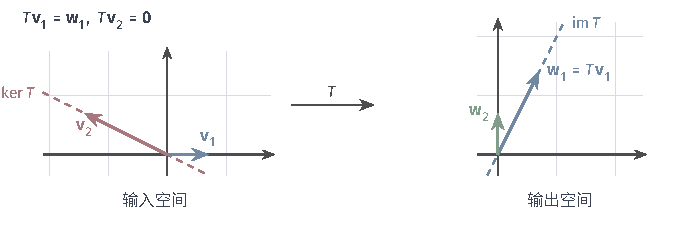
\includegraphics[width=112mm]{figures/00-shared/mathematical-preliminaries-upper/02-linear-spaces/tikz/comprehension-additions/equivalence-two-bases.pdf}
  \caption{两端独立选基化为秩标准形。$T(\bm x)=\bm A\bm x$，$\bm A=\left[\begin{smallmatrix}1&2\\2&4\end{smallmatrix}\right]$。左：输入基$\bm v_1=\bm e_1$（蓝）与$\bm v_2=(-2,1)^{\top}$（红），$\bm v_2$在核（红虚线）上。右：输出基$\bm w_1=T\bm v_1=(1,2)^{\top}$（蓝）位于像（蓝虚线）上，$\bm w_2=\bm e_2$（绿）补足一组基。在这两组基下$T$的矩阵为$\operatorname{diag}(1,0)$。}
  \label{fig:ls-equivalence-two-sided-bases-flow}
\end{figure}

\begin{theorem}[相抵判据]
\label{thm:ls-equivalence-criterion}
两个同形实矩阵$\bm A,\bm B\in\mathbb R^{m\times d}$相抵，当且仅当$\operatorname{rank}\bm A=\operatorname{rank}\bm B$。
\end{theorem}
\begin{proof}
必要性由式\eqref{eq:ls-equivalence-invariants}得到。充分性：设二者秩都为$r$，由上面的构造，存在可逆矩阵使$\bm R=\bm Q_A^{-1}\bm A\bm P_A=\bm Q_B^{-1}\bm B\bm P_B$，其中$\bm R$是式\eqref{eq:ls-rank-normal-form}的秩标准形。两式对接得$\bm B=(\bm Q_A\bm Q_B^{-1})^{-1}\bm A(\bm P_A\bm P_B^{-1})$，即二者相抵。
\end{proof}
所以固定形状以后，秩就是相抵的完整不变量：零矩阵只与零矩阵相抵，同形的满秩矩阵彼此相抵。把矩阵化到标准形的具体消元算法在第~\ref{chap:linear-equations-and-optimization}章建立。

\subsubsection{线性算子的换基与相似}
\label{sec:ls-similarity}
\phantomsection
\label{sec:ls-matrix-equivalences}

线性算子$T:V\to V$的输入与输出是同一个空间，记录时两端用同一组基；换基时，两端必须换成同一组新基。上面的推导加上这个约束会给出什么关系？同一个算子的两个方阵记录什么时候可以互相转化？

\paragraph{换基过程}
设$\mathcal B$与$\mathcal B'$是$V$的两组基，$\bm A=[T]_{\mathcal B}$、$\bm B=[T]_{\mathcal B'}$，记$\bm P=\bm S_{\mathcal B\leftarrow\mathcal B'}$，它的第$j$列是新基向量$\bm b'_j$在旧基$\mathcal B$下的坐标，$\bm P$可逆，反向换基矩阵为$\bm P^{-1}$。输入端与输出端是同一个空间、同一次换基，所以三步推导中的$\bm Q$也是$\bm P$：先把新坐标换成旧坐标，$[\bm v]_{\mathcal B}=\bm P[\bm v]_{\mathcal B'}$；在旧基下作用，$[T\bm v]_{\mathcal B}=\bm A\bm P[\bm v]_{\mathcal B'}$；再把输出换回新坐标，
\[
 [T\bm v]_{\mathcal B'}=\bm P^{-1}[T\bm v]_{\mathcal B}=\bm P^{-1}\bm A\bm P[\bm v]_{\mathcal B'}.
\]
与$[T\bm v]_{\mathcal B'}=\bm B[\bm v]_{\mathcal B'}$逐列比较，得到
\begin{equation}
 \bm B=\bm P^{-1}\bm A\bm P.
 \label{eq:linear-algebra-similarity-change-basis}
\end{equation}
这就是式~\eqref{eq:ls-equivalence-transform}取$\bm Q=\bm P$的情形。

\paragraph{相似的定义}
\phantomsection
\label{sec:ls-similarity-meaning}
与相抵一样，把同一算子两个记录之间的关系单独命名。
\begin{definition}[矩阵相似]
\label{def:ls-matrix-similarity}
设$\bm A,\bm B$是$n$阶方阵。若存在$n$阶可逆矩阵$\bm P$使$\bm B=\bm P^{-1}\bm A\bm P$，就称$\bm A$与$\bm B$\term{相似}（similar）。
\end{definition}
相似的两个矩阵正是同一个线性算子在两组基下的记录。一个方向由上面的推导给出；另一方向，给定$\bm A=[T]_{\mathcal B}$和可逆$\bm P$，以$\bm P$的各列为旧基坐标得到一组新基，$T$在其下的矩阵恰为$\bm P^{-1}\bm A\bm P$。

相似不要求$\bm A,\bm B$本身可逆，可逆的只是换基矩阵$\bm P$。取$\bm Q=\bm P$可见，相似的矩阵必定相抵；反之不然，下面的判定会给出秩相同、因而相抵却不相似的例子。

看一个具体例子：适当换基，可以把一个算子的矩阵化成对角形。
\begin{example}[换基把算子的矩阵化为对角形]
\label{ex:ls-similarity-diagonal}
给定：示例~\ref{ex:ls-plane-operator-matrix}中的算子$T(x_1,x_2)=(2x_1+x_2,3x_2)$，它在标准基下的矩阵为$\bm A=\left[\begin{smallmatrix}2&1\\0&3\end{smallmatrix}\right]$，即$T\bm e_1=2\bm e_1$、$T\bm e_2=\bm e_1+3\bm e_2$；新基取$\bm b_1'=\bm e_1$、$\bm b_2'=\bm e_1+\bm e_2$。

计算：$\bm P=\left[\begin{smallmatrix}1&1\\0&1\end{smallmatrix}\right]$，$\bm P^{-1}=\left[\begin{smallmatrix}1&-1\\0&1\end{smallmatrix}\right]$，
\[
 \bm B=\bm P^{-1}\bm A\bm P
 =\begin{bmatrix}1&-1\\0&1\end{bmatrix}
 \begin{bmatrix}2&1\\0&3\end{bmatrix}
 \begin{bmatrix}1&1\\0&1\end{bmatrix}
 =\begin{bmatrix}2&0\\0&3\end{bmatrix}.
\]
直接验证也是如此：$T\bm b_1'=2\bm b_1'$，$T\bm b_2'=T\bm e_1+T\bm e_2=3\bm e_1+3\bm e_2=3\bm b_2'$。

结论：在新基下，$T$的矩阵是对角矩阵$\operatorname{diag}(2,3)$；两个新基方向在$T$的作用下都只被伸缩、不被转向，彼此互不干扰。
\end{example}
$T$本身没有改变，改变的只是沿哪两条方向读取。图~\ref{fig:ls-similarity-change-of-basis-flow}把这一点画在平面上：在标准基下，单位正方形被$T$拉成一个斜的平行四边形，矩阵$\bm A$有非零的非对角元；在新基下，基向量围成的平行四边形只沿两条基方向分别伸长$2$倍和$3$倍，矩阵就是对角的$\bm B$。只被伸缩的方向称为特征方向；怎样系统地找到它们，什么时候能找到足够多的这种方向组成一组基，是第~\ref{chap:linear-analysis}章的问题。
\begin{figure}[!htb]
  \centering
  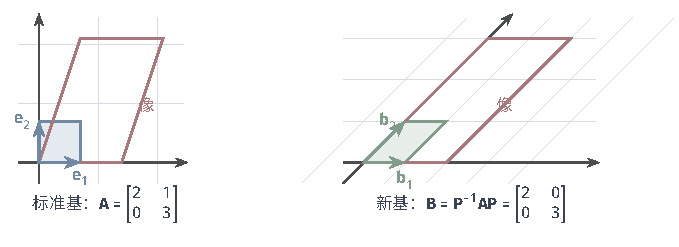
\includegraphics[width=112mm]{figures/00-shared/mathematical-preliminaries-upper/02-linear-spaces/tikz/comprehension-additions/similarity-two-bases.pdf}
  \caption{同一个算子在两组基下的记录。左：标准基$\bm e_1,\bm e_2$围成的单位正方形（蓝）被$\bm A=\left[\begin{smallmatrix}2&1\\0&3\end{smallmatrix}\right]$送到红色平行四边形，形状被斜切。右：新基$\bm b_1=\bm e_1$、$\bm b_2=\bm e_1+\bm e_2$围成的平行四边形（绿）被同一个算子送到红色平行四边形，只沿$\bm b_1$伸长$2$倍、沿$\bm b_2$伸长$3$倍，因此新矩阵为$\operatorname{diag}(2,3)$。浅色斜线为新基网格。}
  \label{fig:ls-similarity-change-of-basis-flow}
\end{figure}

\paragraph{相似不变量}
\phantomsection
\label{sec:ls-similarity-properties}
同一个算子的性质不应随基改变；哪些量在相似下保持不变？相似首先是等价关系：$\bm A=\bm I^{-1}\bm A\bm I$给出自反性；由$\bm B=\bm P^{-1}\bm A\bm P$得$\bm A=\bm P\bm B\bm P^{-1}$，给出对称性；若再有$\bm C=\bm Q^{-1}\bm B\bm Q$，则$\bm C=(\bm P\bm Q)^{-1}\bm A(\bm P\bm Q)$，给出传递性。这三条分别对应不换基、换回原基和连续换两次基。

相似是相抵的特例，相抵不变量自然保持：$\operatorname{null}(\bm B)=\bm P^{-1}\operatorname{null}(\bm A)$，$\operatorname{range}(\bm B)=\bm P^{-1}\operatorname{range}(\bm A)$，因此
\begin{equation}
 \operatorname{rank}\bm B=\operatorname{rank}\bm A,
 \qquad
 \dim\operatorname{null}(\bm B)=\dim\operatorname{null}(\bm A).
 \label{eq:ls-similarity-invariants}
\end{equation}
算子还能反复作用，而先后作用与换基相容：若$\bm B_1=\bm P^{-1}\bm A_1\bm P$、$\bm B_2=\bm P^{-1}\bm A_2\bm P$，则
\begin{equation}
 \bm B_1\bm B_2
 =\bm P^{-1}\bm A_1\bm P\,\bm P^{-1}\bm A_2\bm P
 =\bm P^{-1}\bm A_1\bm A_2\bm P,
 \label{eq:ls-similarity-product}
\end{equation}
中间的$\bm P\bm P^{-1}$相消。归纳得$\bm B^k=\bm P^{-1}\bm A^k\bm P$：反复作用同一个算子，在新基下仍是同一过程的记录。同样，对任意实数$c$，$\bm B-c\bm I=\bm P^{-1}(\bm A-c\bm I)\bm P$，所以$\bm A-c\bm I$与$\bm B-c\bm I$也相似，由式~\eqref{eq:ls-similarity-invariants}，
\begin{equation}
 \operatorname{rank}(\bm B-c\bm I)=\operatorname{rank}(\bm A-c\bm I),\qquad c\in\mathbb R.
 \label{eq:ls-similarity-shifted-rank}
\end{equation}
这比总秩更细：它对每个$c$都给出一个不变量。

相似还保持两个可以直接计算的标量。由行列式的乘法性（第~\ref{sec:ls-determinant-properties}节）与$\det(\bm P^{-1})\det\bm P=\det\bm I=1$，
\[
 \det(\bm P^{-1}\bm A\bm P)=\det(\bm P^{-1})\,\det\bm A\,\det\bm P=\det\bm A;
\]
由迹的循环性（式~\eqref{eq:linear-algebra-trace-cyclic}），
\[
 \operatorname{tr}(\bm P^{-1}\bm A\bm P)=\operatorname{tr}\bigl((\bm A\bm P)\bm P^{-1}\bigr)=\operatorname{tr}\bm A.
\]
两式说明，行列式与迹只依赖算子本身，是判断两个矩阵能否记录同一算子时可以直接计算的两个标量不变量。例如示例~\ref{ex:ls-similarity-diagonal}中的$\bm A$与$\bm B=\operatorname{diag}(2,3)$行列式都是$6$，迹都是$5$。于是可以说“算子$T$的行列式”“算子$T$的迹”，用任意一组基下的矩阵计算即可。

引入特征值以后还将看到（第~\ref{sec:ls-eigen-similarity-invariance}节），特征值与特征多项式同样是相似不变量，而行列式与迹恰好是特征值之积与特征值之和。一般的换基不保持欧氏长度与夹角，这些度量量不在相似保持之列。

\paragraph{相似的判定}
\phantomsection
\label{sec:ls-similarity-conditions}
怎样判断两个给定的方阵是否相似？两端左乘$\bm P$，相似等价于存在\emph{可逆}的$\bm P$满足
\begin{equation}
 \bm A\bm P=\bm P\bm B.
 \label{eq:ls-similarity-equation}
\end{equation}
这是关于$\bm P$各元素的一组线性方程。只找到非零但不可逆的解还不够：那只是两个坐标子空间之间的对应，不是两组基之间的换基。

不变量给出否定的判据：只要某个相似不变量不同，两个矩阵就不相似。但秩、行列式、迹相同，都只是相似的必要条件，下面的例子说明它们合在一起也不够。
\begin{example}[反例：相抵而不相似的两个矩阵]
\label{ex:ls-equivalent-not-similar}
给定：$\bm I_2$与$\bm J=\left[\begin{smallmatrix}1&1\\0&1\end{smallmatrix}\right]$。

验证：二者都可逆，秩都为$2$，由相抵判据它们相抵；二者的行列式都是$1$，迹都是$2$。但取$c=1$，$\bm I_2-\bm I_2=\bm0$的秩为$0$，而$\bm J-\bm I_2=\left[\begin{smallmatrix}0&1\\0&0\end{smallmatrix}\right]$的秩为$1$，式~\eqref{eq:ls-similarity-shifted-rank}不成立。更直接地，若$\bm J=\bm P^{-1}\bm I_2\bm P$，则$\bm J=\bm P^{-1}\bm P=\bm I_2$，矛盾。

结论：$\bm I_2$与$\bm J$相抵，秩、行列式与迹也都相同，却不相似；单位矩阵只与自己相似。
\end{example}
这正是“两端换基相同”这一约束的代价：相抵时秩相同就足够，相似时连秩、行列式与迹一起相同都不够。比较$\bm A-c\bm I$在各个$c$处的秩是更细的必要条件；完整的相似分类需要Jordan标准形，本书不展开。
